\documentclass{article}

\usepackage{graphicx}
\graphicspath{ {../images/} }

\usepackage{hyperref}
\hypersetup{
    colorlinks=true,
    linkcolor=blue,
    filecolor=magenta,      
    urlcolor=cyan,
}
\urlstyle{same}

\usepackage{titlesec}
\titlespacing*{\section}
{0pt}{10ex plus 1ex minus .2ex}{4.3ex plus .2ex}
\titlespacing*{\subsection}
{0pt}{5.5ex plus 1ex minus .2ex}{4.3ex plus .2ex}

\title{Inverse Kinematics of a 12 DOF Quadruped}
\author{Christopher Schicho}
\date{\today}

\begin{document}
    \maketitle
    \tableofcontents
    \pagebreak



    \section{Introduction}
    \paragraph{}  
    This Paper is about the inverse kinematics of a 12 DOF quadruped robot. It is based on an open source project called "open-quadruped". Nevertheless, this paper describes the kinematic in a general way. Therefore, it is useable for other 12 DOF quadruped projects as well. 

    \subsection{Purpose}
    \paragraph{}
    The purpose of this paper is to give you an oversight about what the inverse kinematics is about and to show you, how you use this for your own project. 


    
    \section{3 DOF Leg Inverse Kinematics}
    \paragraph{}
    First things first, let us define what inverse kinematics is about. The key idea of inverse kinematics is to only care about the position of the end of a kinematic chain, the so called end-effector. We do not want to care about all the variable joint parameters needed to reach this position. Therefore, we need to create an algorithm in order to calculate all of these variable joint parameters automatically. 
    \paragraph{}
    This is exactly what this section will discover. We will start with calculating every single axis and combine them to a complete leg inverse kinematics model once we are done with these single steps.
    
    
    %\pagebreak
    \subsection{Z-Axis}
    \paragraph{}
    The easiest way to start is by starting with the z-axis. The z-axis is responsible for moving the quadruped's body up and down. In this step we will calculate the upper leg's and the lower leg's joint angles.

    \paragraph{}
    In order to calculate the necessary joint parameters we need some details about the used quadrupedal robot. For this axis we need to know the length from pivot to pivot of the upper and lower leg. The used measurement unit is not important for this calculation, as long as you use the same for every length / variable. However, usually I suggest using millimeters.

    \paragraph{}
    In the picutre below you can see one of the quadruped's leg and also the triangle we will need in order to calculate our joint parameters. Due to the Design of this model, the end of the lower leg will always be directly under the pivot of the upper leg, but note that this is only true if we only perform z-axis movements. This is a good configuration and makes calculating the angles much easier.
    
    \paragraph{}
    \begin{center}
        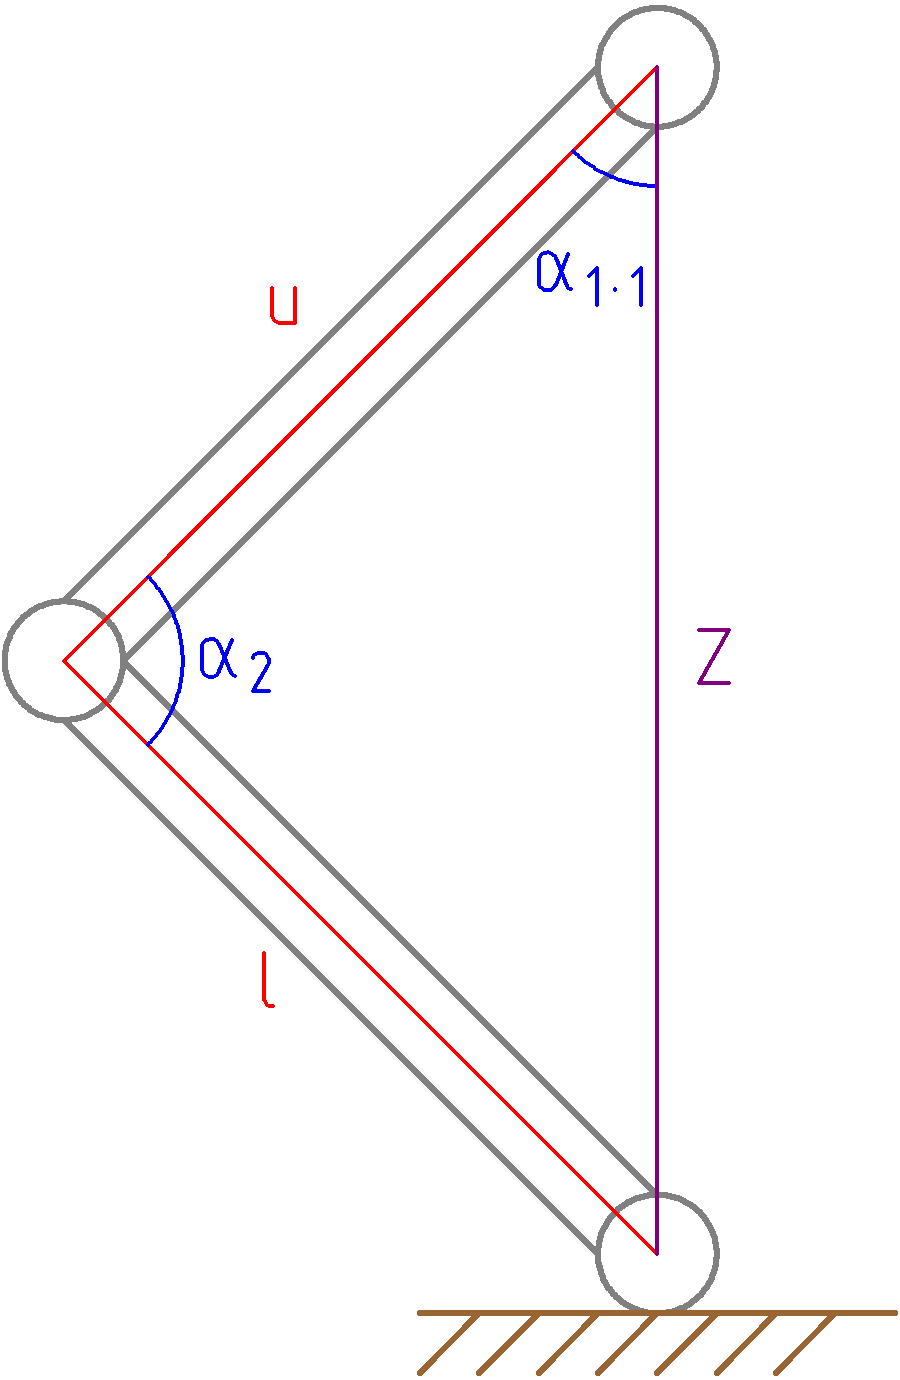
\includegraphics[scale=0.2]{z-axis}
    \end{center}

    \paragraph{}
    The first calculation uses the cosine rule to calculate the angle $\alpha_{1.1}$, where $Z$ is the input for the z-axis, $u$ the length of the upper leg and $l$ the length of the lower leg. This calculation is only directly applied to the quadruped if you want to perform the z-axis movements without including the other axis, otherwise the value of $\alpha_1$ will be calculated in the x-axis step.
    \paragraph{}

    \begin{equation} \label{alpha_1_z}
        \alpha_{1.1} = \arccos \frac{u^2 + Z^2 - l^2}{2 * u * Z} 
    \end{equation}

    \paragraph{}
    The second calculation uses the same rule for calculating $\alpha_2$. This is the angle which will determine the wrist movement later.

    \paragraph{}
    \begin{equation}
        \alpha_2 = \arccos \frac{u^2 + l^2 - Z^2}{2 * u * l} 
    \end{equation}

    \paragraph{}
    At this point we are done with the z-axis calculation. The quadruped is now able to perform movements along the z-axis.



    %\pagebreak
    \subsection{X-Axis}
    \paragraph{} 
    The next step is to calculate the x-axis' parameters. This axis is responsible for moving the body back and forth. In this step we do not need any further information about the quadruped.

    \paragraph{}
    The picture below shows again one leg of the quadrupedal robot, however, this time it looks a litte bit different. Note that x-axis may have positive and negative values. This is slightly different compared to the the z-axis which is only positive. 

    \paragraph{}
    \begin{center}
        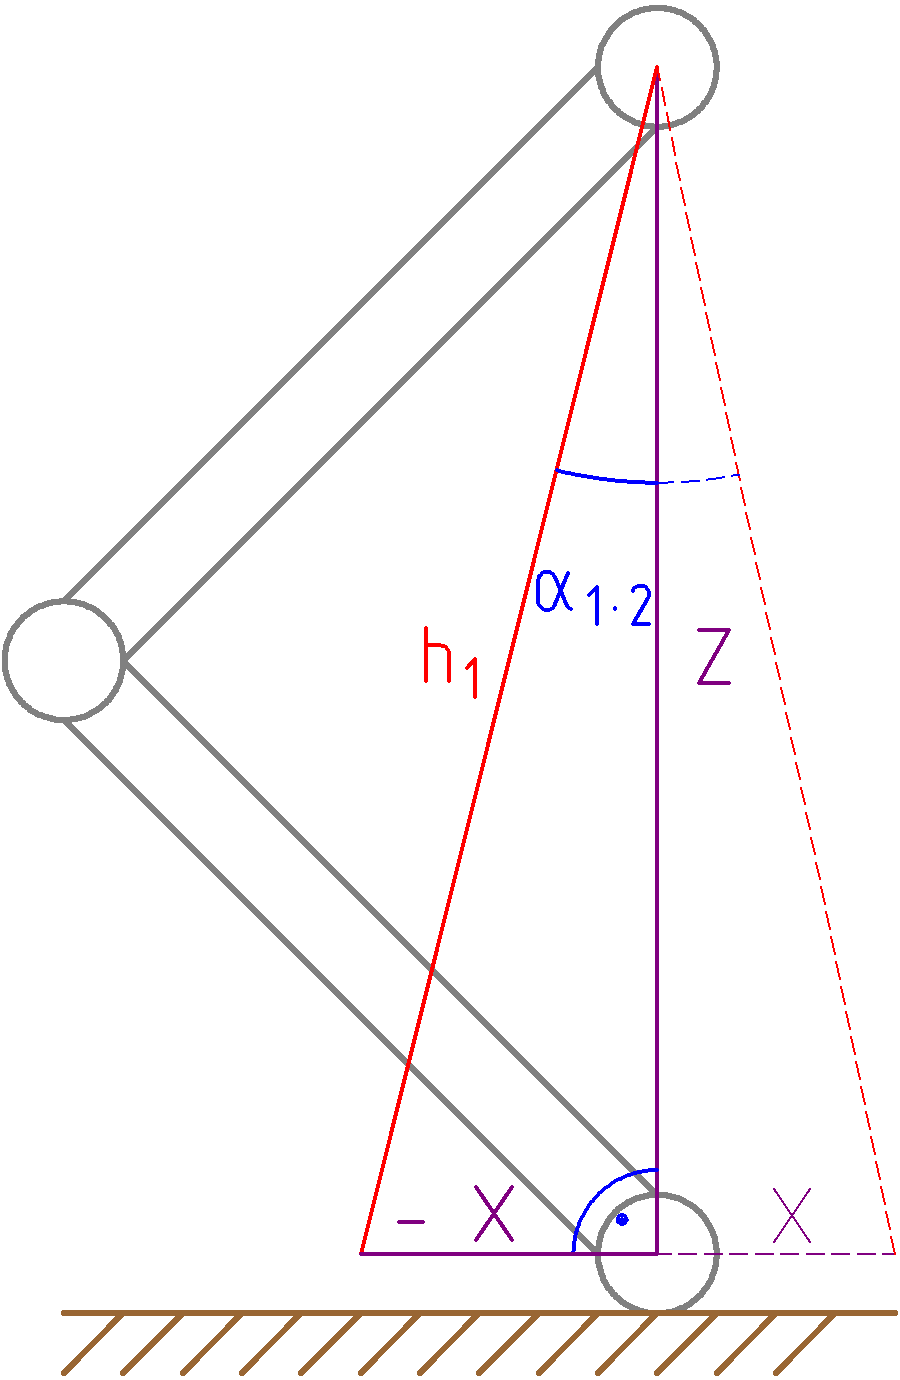
\includegraphics[scale=0.2]{x-axis}
    \end{center}
    
    \paragraph{}
    At first we calculate the hypothenuse from our new triangle by using the Pythagoras theorem. The variables $X$ and $Z$ represent the input for these axis. we will need this length to calculated the desired angle $\alpha_1$.

    \paragraph{}
    \begin{equation}
        h_1 = \sqrt{X^2 + Z^2}
    \end{equation}

    \paragraph{}
    Next we calculate the angle $\alpha_{1.2}$. This angle represents the difference between our desired position and the quadruped's initial position, which we calculated in the z-axis section. 

    \paragraph{}
    \begin{equation}
        \alpha_{1.2} = \arccos \frac{Z}{h_1}
    \end{equation}

    \paragraph{}
    In this step we need to make a case distinction due to the fact that $X$ can be either positive or negative. If $X$ is negative we want to substract $\alpha_{1.2}$ from the initial angle $\alpha_{1.1}$, otherwise we want to add it. We need this step because otherwise the quadruped would only move in one direction. This angle $\alpha_1$ will determine the shoulder movement later.

    \paragraph{}
    \begin{center}
    $\alpha_1 = \left\{
    \begin{array}{ll}
    \alpha_{1.1} + \alpha_{1.2} & \alpha_{1.2} \ge 0 \\
    \alpha_{1.1} - \alpha_{1.2} & \alpha_{1.2} < 0
    \end{array}
    \right. $
    \end{center}

    \paragraph{}
    Now we are also done with the x-axis. At this point we are able to perform movements along the z- and x-axis simultaneously.



    %\pagebreak
    \subsection{Y-Axis}
    \paragraph{} 
    Finally, we will calculate the parameters of the y-axis. This is rather complicated compared to the other ones. This axis is responsible for moving the quadruped's body sidewards.
    
    \paragraph{}
    The following picture illustrates what we will calculate in the next step. The main problem is that if we shift the body sidewards, the legs of one side of the robot get shorter and the other get longer. Therefore we need to calculate two new $Z$ values, we will call them $z_1$ and $z_2$. Furthermore, we will also calculate the angle $alpha_3$ which is our hip angle.

    \paragraph{}
    %\begin{}
    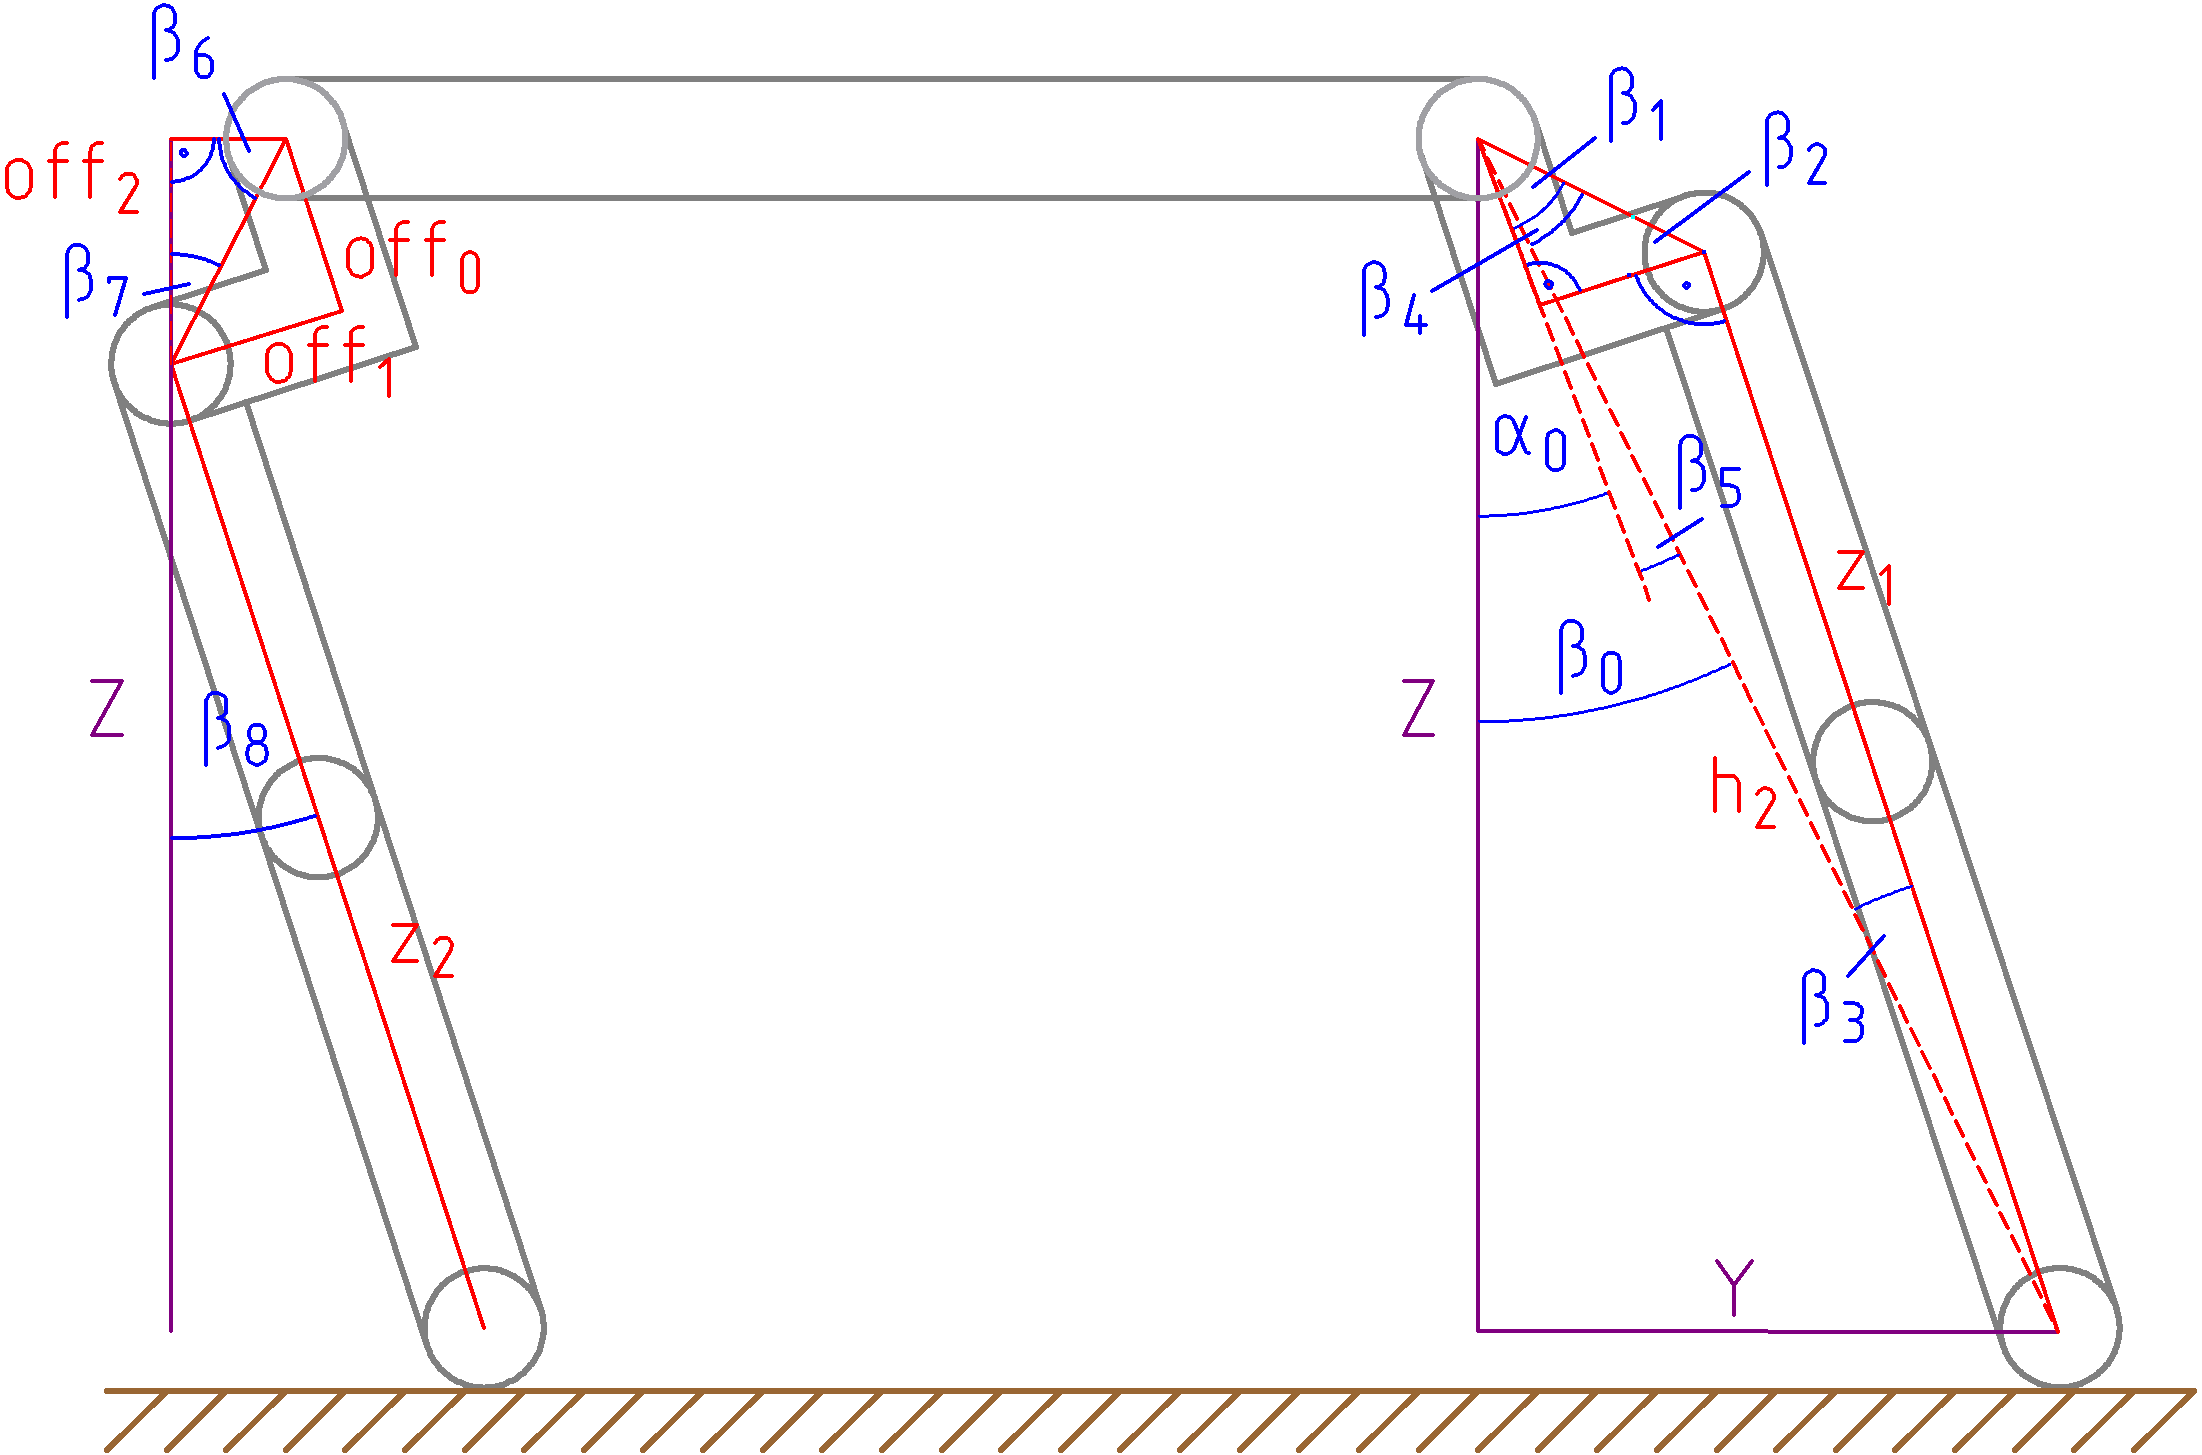
\includegraphics[scale=0.2]{y-axis}
    %\end{center}

    \paragraph{}
    In order to calculate all desired values we need some more details about the construction of the quadruped. As you can see in the picture above we need 2 lengths of the hip joint, we will call them $off_o$ and $off_1$. $off_0$ is the vertical distance between the middle of the hip pivot and the shoulder pivot. $off_1$ is the horizontal distance between the hip pivot and the middle of the upper leg. In order to make the robot's leg standing straight we need to include the $off_1$ to our $Y_{input}$. Also keep in mind that the the y-axis can also be either positive or negative.

    \paragraph{}
    \begin{equation}
        Y = Y_{input} + off_1
    \end{equation}

    \paragraph{}
    We start by calculating some lengths of the triangles and their corresponding angles.

    \paragraph{}
    \begin{equation}
        h_2 = \sqrt{Z^2 + Y^2}
    \end{equation}

    \paragraph{}
    \begin{equation}
        h_3 = \sqrt{off_0^2 + off_1^2}
    \end{equation}

    \paragraph{}
    \begin{equation}
        \beta_0 = \arctan \frac{Y}{Z}
    \end{equation}

    \paragraph{}
    \begin{equation}
        \beta_1 = \arctan \frac{off_1}{0ff_0}
    \end{equation}

    \paragraph{}
    \begin{equation}
        \beta_2 = \arctan \frac{off_0}{off_1}
    \end{equation}

    \paragraph{}
    \begin{equation}
        \beta_3 = \arcsin \frac{h_3 * \sin(\beta_2 + 90)}{h_2}
    \end{equation}

    \paragraph{}
    \begin{equation}
        \beta_4 = 90 - (\beta_2 + \beta_3)
    \end{equation}

    \paragraph{}
    \begin{equation}
        \beta_5 = \beta_1 - \beta_4
    \end{equation}

    \paragraph{}
    The following calculation returns $alpha_0$, which is the hip angle. 

    \paragraph{}
    \begin{equation}
        alpha_0 = \beta_0 - \beta_5
    \end{equation}

    \paragraph{}
    The following steps are necessary to calculate the two different $Z$ values. These values are necessary to execute the calculations of the x- and z-axis.

    \paragraph{}
    \begin{equation}
        \beta_6 = 90 - (\beta_1 - \alpha_0)
    \end{equation}

    \paragraph{}
    \begin{equation}
        \beta_7 = 90 - \beta_6
    \end{equation}

    \paragraph{}
    \begin{equation}
        \beta_8 = 90 - (\beta_6 + \beta_7)
    \end{equation}

    \paragraph{}
    \begin{equation}
        off_2 = h_3 * \cos(\beta_7)
    \end{equation}

    \paragraph{}
    \begin{equation}
        z_1 = \frac{h_3 * \sin(\beta_4)}{\sin(\beta_8)}
    \end{equation}

    \paragraph{}
    \begin{equation}
        z_2 = \frac{Z - off_2}{\cos(\beta_8)}
    \end{equation}

    \paragraph{}
    In case that $Y$ is negative we will use $z_1$ for the right side of the quadruped and $z_2$ for the left side, otherwise we use them the other way around.

    \paragraph{}
    Now we are done with all the calculations. The next step is to combine all this calculations to a final model. 
    


    %\pagebreak
    \subsection{Final Leg Model}
    \paragraph{}
    Due to the two different $Z$ values from the y-axis calculations, we need to replace the calculations of the x- and z-axis by the following functions. We will use this calculations additionally to the y-axis calculations. Basically we need to distinguish if we are calculating the left or the right side of the quadruped. Therefore, we will introduce some new angles, namely $\alpha_{1left}$, $\alpha_{1right}$, $\alpha_{2left}$, $\alpha_{2right}$, $\alpha_{1.1left}$, $\alpha_{1.1right}$, $\alpha_{1.2left}$ and $\alpha_{1.2right}$ and some new lenghts.

    \paragraph{}
    \begin{center}
    $\alpha_{1.1left} = \left\{
    \begin{array}{ll}
    \arccos \frac{u^2 + z_1^2 - l^2}{2 * u * z_1} & Y \ge 0 \\ \\
    \arccos \frac{u^2 + z_2^2 - l^2}{2 * u * z_2} & Y < 0 
    \end{array}
    \right. $ 

    \paragraph{}
    $\alpha_{1.1right} = \left\{
    \begin{array}{ll}
    \arccos \frac{u^2 + z_2^2 - l^2}{2 * u * z_2} & Y \ge 0 \\ \\
    \arccos \frac{u^2 + z_1^2 - l^2}{2 * u * z_1} & Y < 0
    \end{array}
    \right. $ 

    \paragraph{}
    $\alpha_{1.2left} = \left\{
    \begin{array}{ll}
    \arccos \frac{z_1}{\sqrt{X^2 + z_1^2}} & Y \ge 0 \\ \\
    \arccos \frac{z_2}{\sqrt{X^2 + z_2^2}} & Y < 0
    \end{array}
    \right. $ 

    \paragraph{}
    $\alpha_{1.2right} = \left\{
    \begin{array}{ll}
    \arccos \frac{z_2}{\sqrt{X^2 + z_2^2}} & Y \ge 0 \\ \\
    \arccos \frac{z_1}{\sqrt{X^2 + z_1^2}} & Y < 0
    \end{array}
    \right. $ 

    \paragraph{}
    $\alpha_{1left} = \left\{
    \begin{array}{ll}
    \alpha_{1.1left} + \alpha_{1.2left} & \alpha_{1.2left} \ge 0 \\ \\
    \alpha_{1.1left} - \alpha_{1.2left} & \alpha_{1.2left} < 0
    \end{array}
    \right. $    

    \paragraph{}
    $\alpha_{1right} = \left\{
    \begin{array}{ll}
    \alpha_{1.1right} + \alpha_{1.2right} & \alpha_{1.2right} \ge 0 \\ \\
    \alpha_{1.1right} - \alpha_{1.2right} & \alpha_{1.2right} < 0
    \end{array}
    \right. $   

    \paragraph{}
    $\alpha_{2left} = \left\{
    \begin{array}{ll}
    \arccos \frac{u^2 + l^2 - z_1^2}{2 * u * l} & Y \ge 0 \\ \\
    \arccos \frac{u^2 + l^2 - z_2^2}{2 * u * l} & Y < 0
    \end{array}
    \right. $   

    \paragraph{}
    $\alpha_{2right} = \left\{
    \begin{array}{ll}
    \arccos \frac{u^2 + l^2 - z_2^2}{2 * u * l} & Y \ge 0 \\ \\
    \arccos \frac{u^2 + l^2 - z_1^2}{2 * u * l} & Y < 0
    \end{array}
    \right. $  
    \end{center}

    \paragraph{}
    At this point we are done with the 3 DOF leg inverse kinematics of a 12 DOF quadrupedal robot. The calculations above are all you need in order to move a a robot along the x-, y- and z-axis. 



    \section{Body Inverse Kinematics}
    \paragraph{}
    COMING SOON!

    %\subsection{Pitch}
    %\paragraph{}

    %\subsection{Yaw}
    %\paragraph{}

    %\subsection{Roll}
    %\paragraph{}

    %\subsection{Final Body Model}
    %\paragraph{}



    \section{Outroduction}
    \paragraph{}
    At this point we are done with all the calculations. Our Quadruped is now able to perform all necessary movements except walking. The next step will be to make the quadruped walk. Therefore, dynamic walking will be subject of the next paper.
    \paragraph{}
    In case that you are interested in the project or how all of this works applied to a real robot. Then just visit the following sites: \\
    \url{www.enabling-intelligence.com} \\
    \url{https://github.com/c-schicho}



    \section{References}
    \url{https://en.wikipedia.org/wiki/Inverse_kinematics} \\
    \url{https://www.adham-e.dev/pdf/IK_Model.pdf} \\
    \url{https://github.com/adham-elarabawy/open-quadruped}



\end{document}